\section{Middlware, communications patterns and their applications}

In a distributed system, we view middleware as one or multiple applications that homogenize and simplifies the communication and integration between nodes. It is suitable to link systems of various origin and to institute so-called "plumbing", but may add complexity and extra cost to the design and additional overhead, as data from the application-layer (user-space) has to traverse a extra layer of middleware protocols before being put on a wire or broadcasted to its destination. This is seen in figure \ref{fig:middleware}. 

\begin{figure}[h!]\label{}
	\centering
	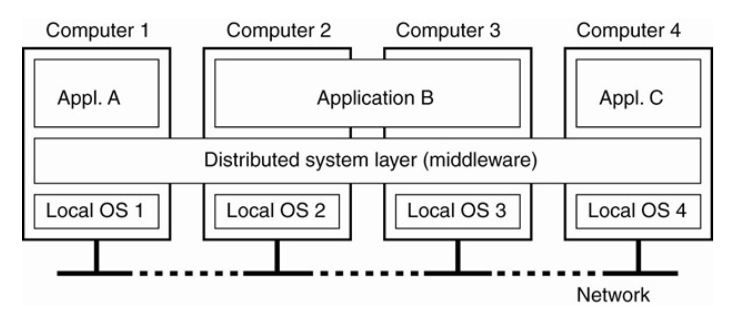
\includegraphics[scale=0.5]{middleware/middlewaredist.png}
	\caption{Middleware in a distributed system, situtaed between the application layer and the internal part of the local operating system.}
	\label{fig:middleware}
\end{figure}

Examples of modern middleware includes Postscript printing, the IEEE TCP/IP protocol, database tools like Microsoft's OLEDB, ADO.NET and Entity Framework for SQL operations, the CSharp language and underlying .NET runtime framework, and more especially the DDS standard, which we will discuss in the next section. Whichever middleware application we consider, they offer various traits in a distributed system. We look at three key ones, space, time and flow decoupling:

\textbf{Space}: Producers and consumers do not know each-other and no direct link exist.

\textbf{Time}: Communication is asynchronous. A producer or consumer does not have to block and wait on the counterpart.

\textbf{Flow}: The data production and consumption does not reside in the main flow of the producer or the consumer, i.e. they have additional threads or loops to handle calls.

Decoupling removes the implied dependency between producer and consumer, when communications occur. These decoupling traits are important when examining middleware applications and its communication-patterns.




